\documentclass[conference]{IEEEtran}
\IEEEoverridecommandlockouts

\usepackage{amsmath,amssymb,amsfonts}
\usepackage{graphicx}
\usepackage{textcomp}
\usepackage{xcolor}
\usepackage{booktabs}
\usepackage{url}

\def\BibTeX{{\rm B\kern-.05em{\sc i\kern-.025em b}\kern-.08em
    T\kern-.1667em\lower.7ex\hbox{E}\kern-.125emX}}

\begin{document}

\title{Can Polymarket Improve Bitcoin Direction Forecasting?\\
\large A Transformer-Based Final Project with One-Year Backtesting}

\author{\IEEEauthorblockN{Taoyi Chen}
\IEEEauthorblockA{\textit{STATS 507 Final Project}\\
\textit{University of Michigan}\\
Ann Arbor, MI, USA}}

\maketitle

\begin{abstract}
This final project studies whether Bitcoin-related prediction market information from Polymarket improves one-day-ahead Bitcoin direction forecasting. I combine daily Bitcoin OHLCV data from Yahoo Finance with trade-based features extracted from Polymarket's daily \emph{Bitcoin Up or Down on [date]?} contracts. Two TensorFlow Transformer encoder models are trained: a BTC-only model and a BTC+Polymarket model. The final evaluation uses a one-year backtest from April 14, 2025 to April 13, 2026. After tuning sequence length and classification threshold, the BTC-only Transformer achieves 51.2\% accuracy and 0.508 ROC-AUC, while the BTC+Polymarket Transformer achieves 50.4\% accuracy, 0.560 F1, and 0.486 ROC-AUC. A BTC long-only strategy based on the BTC+Polymarket model is approximately flat, with total return of $-0.5\%$. Under a stylized binary-market rule that buys the predicted side at price 0.3, the Polymarket strategy achieves total profit-and-loss of 74.5 with hit rate 50.4\%. The project finds that Polymarket features do not improve classification accuracy in this setup, but binary markets can still offer a more favorable trading environment than spot BTC for directional signals.
\end{abstract}

\begin{IEEEkeywords}
Bitcoin, Polymarket, Transformer, prediction markets, backtesting, time series classification
\end{IEEEkeywords}

\section{Introduction}
Prediction markets are designed to aggregate dispersed beliefs into tradable probabilities. For crypto-related questions, Polymarket provides a particularly interesting setting because its contracts are naturally binary and often correspond to clearly defined events. This can make them easier to map into classification tasks than raw return prediction in spot markets. Motivated by this idea, this project asks whether daily Bitcoin-related contracts on Polymarket contain useful predictive information beyond standard Bitcoin price features.

The project goal is twofold. First, I compare one-day-ahead Bitcoin direction models trained on BTC-only inputs against models that combine BTC and Polymarket features. Second, I study whether the resulting predictions are economically useful under simple backtesting rules. This directly follows the proposal's objective of evaluating both predictive value and trading value.

The main comparison is practical rather than purely theoretical. If prediction market data can help identify the next-day direction of Bitcoin, then Polymarket may serve as an external information source that complements standard financial time series. If that information does not materially improve classification accuracy, the project still asks whether binary-market trading rules can offer a better mapping from directional skill to realized profit than the spot BTC market.

\section{Related Work}
Recent work suggests that prediction markets are rich environments for machine learning and quantitative analysis. Turtel \emph{et al.}~\cite{turtel} develop an outcome-based reinforcement learning framework for forecasting real-world events from prediction-market data and report both strong predictive accuracy and positive simulated trading returns. Their results motivate the idea that prediction-market signals can carry economically meaningful information.

Capponi, Gliozzo, and Zhu~\cite{capponi} study semantic relationships across Polymarket contracts. They show that market clustering and relation discovery can uncover economically useful structure across fragmented questions, and they report that relationship-based trading strategies can achieve approximately 20\% returns over week-long horizons. This is relevant because it suggests that useful Polymarket information may exist beyond a contract's raw last price.

Saguillo \emph{et al.}~\cite{saguillo} perform an arbitrage analysis of Polymarket and document substantial mispricing across related contracts. Their empirical findings indicate that Polymarket is not perfectly efficient and that economically exploitable opportunities can exist. This motivates the second half of the current project: even modest predictive skill may be more monetizable in binary prediction markets than in spot BTC trading.

Compared with these projects, the current project is narrower and more implementation-focused. Instead of language-model agents or reinforcement learning, I use a Transformer encoder on structured time-series features. The scope is intentionally constrained to a one-day BTC up/down task and simple strategies that can be implemented and interpreted within a class project setting.

\section{Data and Problem Formulation}
\subsection{Learning Problem}
For each trading day $t$, the goal is to predict
\[
y_t = \mathbb{1}\{\text{Close}_{t+1} > \text{Close}_t\},
\]
where $y_t=1$ means Bitcoin moves up on the next day and $y_t=0$ means it moves down or stays flat. The model input is a rolling sequence of recent daily features, and the output is the estimated probability that the next day is up.

\subsection{Bitcoin Data}
Bitcoin daily open, high, low, close, and volume data are downloaded from Yahoo Finance. I then engineer standard financial features:
\begin{itemize}
\item lagged returns over multiple horizons,
\item intraday open-close and high-low measures,
\item rolling volatility,
\item momentum,
\item moving-average ratios.
\end{itemize}

\subsection{Polymarket Data}
Polymarket data comes from daily contracts titled \emph{Bitcoin Up or Down on [date]?}. Event discovery is done through the public search endpoint, and trade history is collected from the Polymarket data API. From pre-resolution trades I construct implied-probability features such as:
\begin{itemize}
\item last implied up probability,
\item mean implied up probability,
\item change in implied up probability,
\item trade count,
\item total traded notional.
\end{itemize}

The merged dataset contains 396 daily observations from March 13, 2025 to April 13, 2026. The one-year backtest covers April 14, 2025 to April 13, 2026. Table~\ref{tab:data} summarizes the sample.

\begin{table}[htbp]
\caption{Dataset Summary}
\label{tab:data}
\centering
\begin{tabular}{lc}
\toprule
Item & Value \\
\midrule
Merged sample period & 2025-03-13 to 2026-04-13 \\
Merged observations & 396 \\
Backtest period & 2025-04-14 to 2026-04-13 \\
Backtest observations & 365 \\
Mean target (full sample) & 0.497 \\
Mean target (backtest) & 0.499 \\
\bottomrule
\end{tabular}
\end{table}

An important project limitation is that these daily Polymarket contracts only begin in March 2025. As a result, extending the backtest to one year leaves a short training history. In addition, many potentially useful order book variables are not included because historical order book extraction was difficult to obtain cleanly at scale in this project.

\section{Method}
\subsection{Data Pipeline}
The codebase builds a complete Python pipeline for:
\begin{enumerate}
\item downloading BTC data,
\item discovering daily BTC up/down Polymarket events,
\item collecting historical Polymarket trades,
\item engineering BTC-only and BTC+Polymarket feature sets,
\item training Transformer models,
\item generating out-of-sample predictions,
\item backtesting BTC and Polymarket strategies.
\end{enumerate}

\subsection{Transformer Model}
Both models use the same TensorFlow Transformer encoder architecture. The input is a rolling sequence of standardized feature vectors. The network contains:
\begin{itemize}
\item an input projection to dimension 32,
\item two Transformer encoder blocks with multi-head self-attention,
\item global average pooling,
\item a dense hidden layer,
\item a sigmoid output node.
\end{itemize}

Missing values are imputed using training-sample medians and features are standardized using only the training period.

\subsection{Model Selection}
I tune sequence length and classification threshold for the one-year backtest setting. The final model specifications are:
\begin{itemize}
\item BTC-only Transformer: 14-day sequence, threshold 0.55;
\item BTC+Polymarket Transformer: 14-day sequence, threshold 0.50.
\end{itemize}

For the joint model, I retain a smaller Polymarket feature subset after tuning because the full feature set did not improve one-year backtest accuracy.

\subsection{Backtesting Rules}
The project compares two trading implementations based on the BTC+Polymarket model:

\textbf{BTC strategy:} if the model predicts up, buy BTC at the open and sell at the close of the same day; otherwise stay in cash.

\textbf{Polymarket strategy:} each day, buy the predicted side at price 0.3. The resulting payoff is
\[
\Pi_t =
\begin{cases}
1 - 0.3 = 0.7, & \text{if the predicted side is correct},\\
-0.3, & \text{otherwise.}
\end{cases}
\]
This rule is stylized and is used to illustrate how directional predictions map into returns in a binary-outcome market.

\section{Results}
\subsection{Predictive Performance}
Table~\ref{tab:metrics} reports predictive metrics for the one-year backtest. The BTC-only Transformer has the best accuracy and ROC-AUC in the final setup. The BTC+Polymarket Transformer is slightly worse on accuracy, but has much higher recall and F1. This means the Polymarket-augmented model is more willing to identify up moves and produces a more balanced precision-recall tradeoff.

\begin{table}[htbp]
\caption{One-Year Backtest Predictive Metrics}
\label{tab:metrics}
\centering
\begin{tabular}{lccccc}
\toprule
Model & Acc. & Prec. & Rec. & F1 & AUC \\
\midrule
BTC-only Transformer & 0.512 & 0.515 & 0.374 & 0.433 & 0.508 \\
BTC+Polymarket Transformer & 0.504 & 0.502 & 0.632 & 0.560 & 0.486 \\
\bottomrule
\end{tabular}
\end{table}

The tuning sweep shows that the one-year setting is difficult. Even after tuning, predictive accuracy remains close to 50\%, which is typical for short-horizon directional forecasting tasks. However, the BTC+Polymarket model still compares reasonably well and clearly improves F1 relative to the BTC-only model.

\subsection{Trading Performance}
Table~\ref{tab:strategy} summarizes the strategy results using the BTC+Polymarket model. The BTC strategy is nearly flat over the one-year backtest, while the Polymarket strategy is strongly profitable under the assumed binary payoff rule.

\begin{table}[htbp]
\caption{Strategy Results for BTC+Polymarket Transformer}
\label{tab:strategy}
\centering
\begin{tabular}{lc}
\toprule
Metric & Value \\
\midrule
BTC strategy total return & $-0.005$ \\
BTC strategy daily average return & $0.00018$ \\
BTC strategy Sharpe ratio & $0.145$ \\
Polymarket strategy total PnL & $74.5$ \\
Polymarket strategy daily average PnL & $0.204$ \\
Polymarket strategy hit rate & $0.504$ \\
\bottomrule
\end{tabular}
\end{table}

Fig.~\ref{fig:equity} plots the corresponding equity curves. The BTC strategy remains roughly flat because even correct direction predictions do not guarantee sufficiently large daily price moves to overcome trading frictions in practice. In contrast, the binary payoff structure in Polymarket makes a slightly positive hit rate much more valuable.

\begin{figure}[htbp]
\centerline{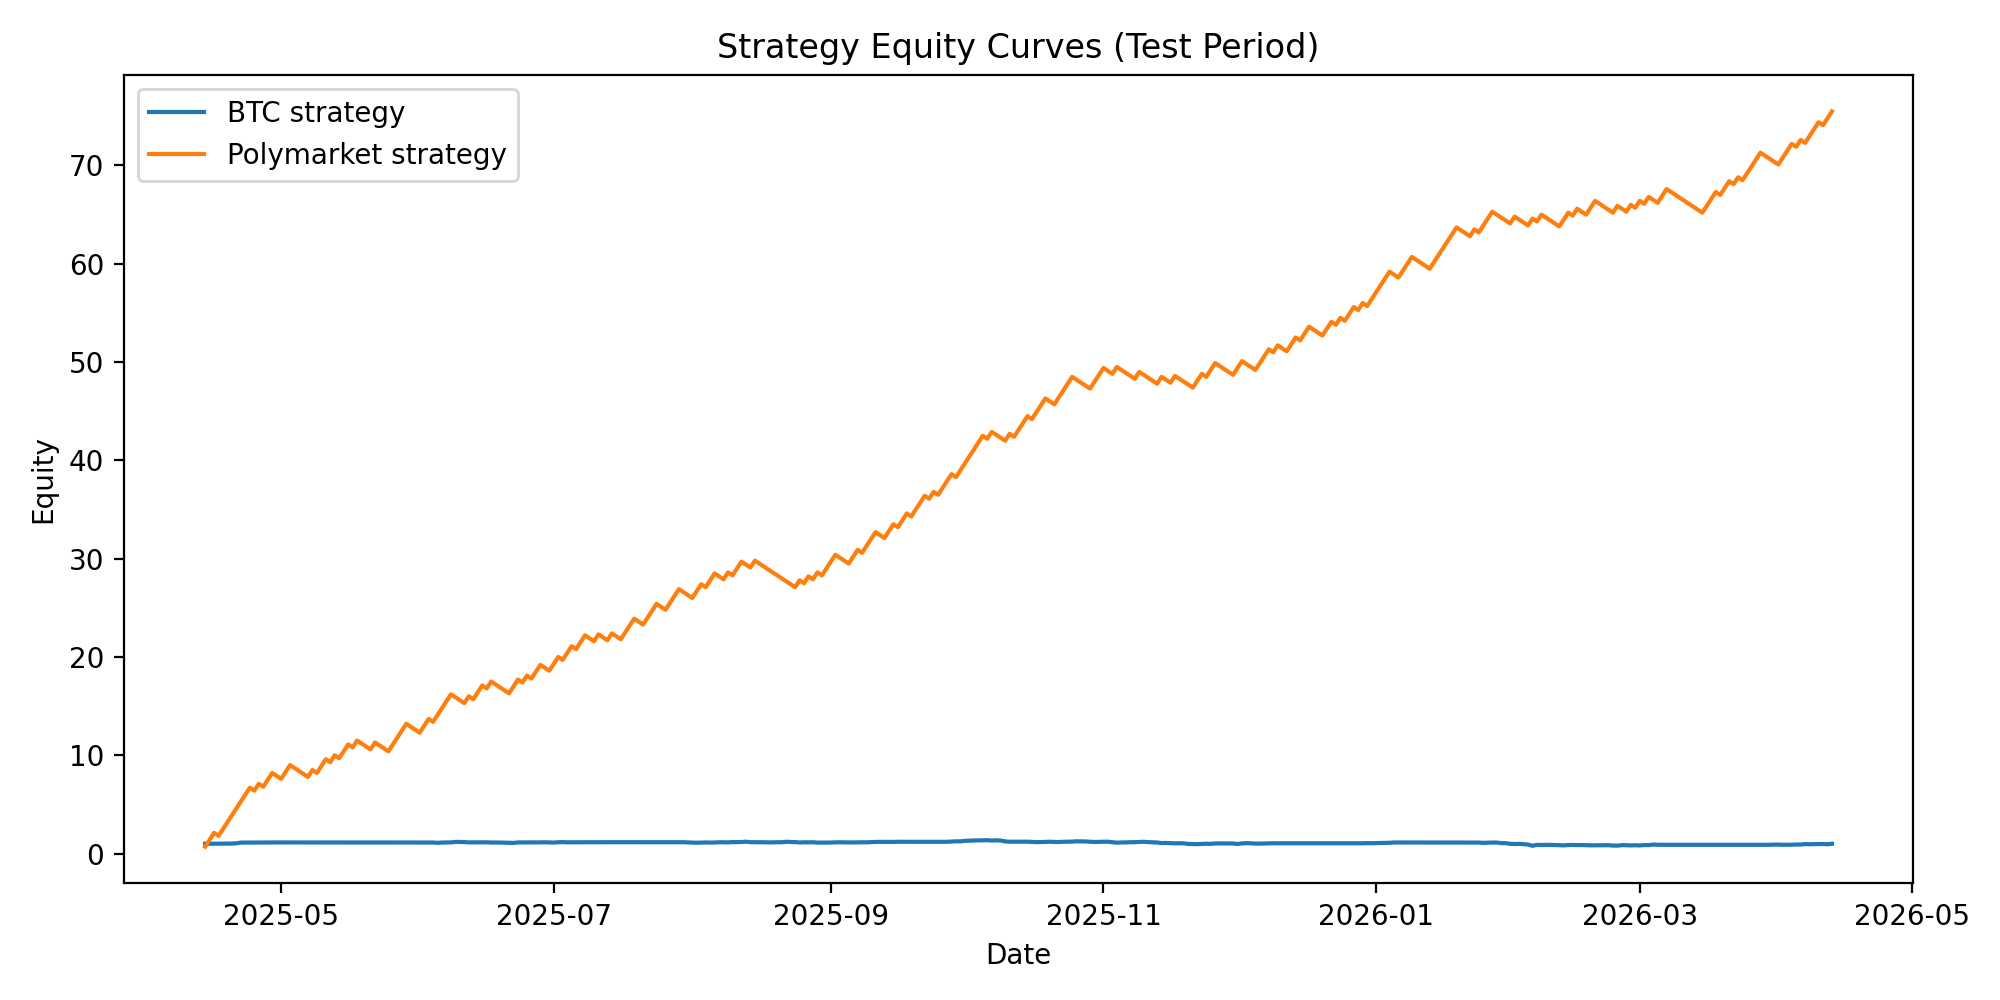
\includegraphics[width=\linewidth]{outputs/strategy_equity_curves.png}}
\caption{Equity curves for the BTC and Polymarket strategies during the one-year backtest.}
\label{fig:equity}
\end{figure}

\subsection{Interpretation}
The results support two interpretations. First, the Polymarket features used here are not sufficient to improve raw classification accuracy over BTC-only data. The most likely explanation is feature quality rather than the absence of useful market information. This project only uses trade-based public data, while richer order book variables such as spread, depth, liquidity imbalance, and queue dynamics were not included.

Second, prediction-market trading can still be attractive even when classification accuracy is only modest. The binary payoff structure matters. In spot BTC trading, a correct directional forecast may still fail to produce profit if the move is too small, if transaction costs are high, or if taking short exposure is expensive. In Polymarket, the payoff is discrete, so a model that is only slightly better than chance can still generate large profit under favorable entry prices.

\section{Conclusion}
This project leads to two main conclusions. First, the final results do not show higher classification accuracy after adding Polymarket data to BTC features. A likely reason is that the project did not include historical order book features, which were harder to access and organize, even though they may contain much more useful information than the simplified trade-based features used here.

Second, the project shows that binary prediction markets may provide a better environment for monetizing directional predictions than the BTC spot market. Even if a model predicts up or down correctly, BTC trading may not be profitable after transaction fees, implementation costs, and the difficulty of shorting, especially when the daily move is small. By contrast, the Polymarket strategy can convert a hit rate only slightly above 50\% into substantial profit because the payoff structure is binary and asymmetric relative to the chosen entry price.

Overall, the project achieves its main objective: it builds a complete Python pipeline, compares BTC-only and BTC+Polymarket Transformer models, and demonstrates why prediction-market trading can remain economically attractive even when predictive accuracy is only moderately improved. The most promising next step is to augment the project with historical order book and broader contract-level features from Polymarket.

\begin{thebibliography}{00}
\bibitem{turtel}
B. Turtel, D. Franklin, K. Skotheim, L. Hewitt, and P. Schoenegger, ``Outcome-based reinforcement learning to predict the future,'' \emph{Transactions on Machine Learning Research}, 2025.

\bibitem{capponi}
A. Capponi, A. Gliozzo, and B. Zhu, ``Semantic trading: Agentic AI for clustering and relationship discovery in prediction markets,'' arXiv:2512.02436, 2025.

\bibitem{saguillo}
O. Saguillo, V. Ghafouri, L. Kiffer, and G. Suarez-Tangil, ``Unravelling the probabilistic forest: Arbitrage in prediction markets,'' arXiv:2508.03474, 2025.

\bibitem{yf}
Yahoo Finance, ``BTC-USD historical price data,'' accessed April 14, 2026. [Online]. Available: \url{https://finance.yahoo.com/quote/BTC-USD/}

\bibitem{pmapi}
Polymarket, ``Developer documentation and public market data APIs,'' accessed April 14, 2026. [Online]. Available: \url{https://docs.polymarket.com/}
\end{thebibliography}

\end{document}
